\documentclass[12pt]{article}
\def\activityid{F05-M-v2}\usepackage[letterpaper,margin=.65in,top=.60in,bottom=.65in]{geometry}
\usepackage[T1]{fontenc}\usepackage[default]{sourcesanspro}
\usepackage{microtype,tikz,array,tabularx,fancyhdr,amsmath}\usepackage[hidelinks]{hyperref}
\usetikzlibrary{arrows.meta,calc}
\setlength{\parindent}{0pt}\setlength{\parskip}{7pt}\setlength{\headheight}{0pt}\setlength{\footskip}{26pt}\setlength{\emergencystretch}{2em}
\pagestyle{fancy}\fancyhf{}\renewcommand{\headrulewidth}{0pt}\renewcommand{\footrulewidth}{.4pt}
\fancyfoot[L]{\scriptsize Bellingham Math Circle / Week 5 / \activityid}\fancyfoot[R]{\scriptsize \thepage}
\definecolor{ink}{gray}{.12}\definecolor{soft}{gray}{.95}\color{ink}
\newcommand{\PageTitle}[2]{{\fontsize{10}{12}\selectfont\bfseries WEEK 5\quad TOWER LAB\hfill #1\par}\vspace{3pt}{\fontsize{26}{29}\selectfont\bfseries #2\par}\vspace{2pt}}
\newcommand{\NameLine}{{\small Name: \rule{2.65in}{.4pt}\hfill Date: \rule{1.35in}{.4pt}\par}\vspace{4pt}}
\newcommand{\Task}[2]{\par\vspace{3pt}{\large\bfseries #1}\par #2\par}
\newcommand{\Subhead}[1]{\par\vspace{3pt}{\large\bfseries #1}\par}
\newcommand{\RuleBox}[1]{\par\begingroup\setlength{\fboxsep}{8pt}\colorbox{soft}{\parbox{\dimexpr\linewidth-16pt\relax}{#1}}\endgroup\par}
\newcommand{\WriteBox}[2]{\par\textbf{#1}\par\vspace{2pt}\begin{tikzpicture}\draw[black!40,line width=.5pt] (0,0) rectangle (\dimexpr\linewidth-.5pt\relax,#2);\end{tikzpicture}\par}
\newcommand{\StudentFooter}{\vfill{\small Build first. Explain by pointing, talking, or drawing.}\par}
\newcommand{\Code}[1]{\texttt{#1}}

\hypersetup{pdftitle={Week 5: grades-2-3}}
\begin{document}
\PageTitle{GRADES 2--3}{One clue, two cities?}\NameLine
\RuleBox{Use heights 1, 2, 3 once in each row and once in each column. A number outside counts towers seen from that end; taller towers hide shorter ones.}
\Task{1. Build a city.}{First make any legal city with your towers. Then add the clue shown here: three towers must be visible down the first column.}\begin{center}\begin{minipage}{.47\linewidth}\centering \begin{tikzpicture}[x=0.7in,y=0.7in]\draw[step=1,black!55] (0,0) grid (3,3);\draw[thick](0,0)rectangle(3,3);\node[font=\bfseries] at (0.5,3.5){3};\end{tikzpicture}\end{minipage}\hfill\begin{minipage}{.47\linewidth}\centering \begin{tikzpicture}[x=0.7in,y=0.7in]\draw[step=1,black!55] (0,0) grid (3,3);\draw[thick](0,0)rectangle(3,3);\node[font=\bfseries] at (0.5,3.5){3};\end{tikzpicture}\end{minipage}\end{center}
\Task{2. Find every city with that clue.}{Record two different cities above. Are there more? Keep the board in the same orientation.}
\WriteBox{Explain why your list is complete. What can go in the top row?}{1.05in}
\textbf{Hint after trying:} The first column is forced. Try each possible order of the two remaining heights in the top row.\StudentFooter
\newpage
\PageTitle{GRADES 2--3}{How little information is enough?}\NameLine
\Task{3. Make just one city possible.}{Keep the top clue 3. Add a right-side clue of 2 to the \textbf{middle row}. Which of your two cities survives? Show why.}\begin{center}\begin{tikzpicture}[x=0.7in,y=0.7in]\draw[step=1,black!55] (0,0) grid (3,3);\draw[thick](0,0)rectangle(3,3);\node[font=\bfseries] at (3.5,1.5){2};\node[font=\bfseries] at (0.5,3.5){3};\end{tikzpicture}\end{center}
\Task{4. Is either clue unnecessary?}{Cover the right clue: your first page gives two answers. Now cover only the top clue. Find two cities that keep the right clue.}
\begin{center}\begin{minipage}{.47\linewidth}\centering 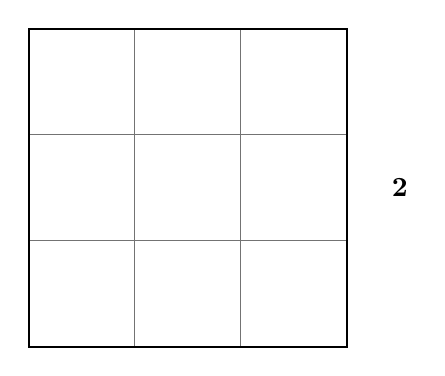
\begin{tikzpicture}[x=0.53in,y=0.53in]\draw[step=1,black!55] (0,0) grid (3,3);\draw[thick](0,0)rectangle(3,3);\node[font=\bfseries] at (3.5,1.5){2};\end{tikzpicture}\end{minipage}\hfill\begin{minipage}{.47\linewidth}\centering 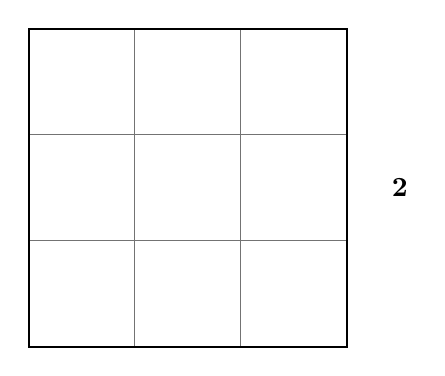
\begin{tikzpicture}[x=0.53in,y=0.53in]\draw[step=1,black!55] (0,0) grid (3,3);\draw[thick](0,0)rectangle(3,3);\node[font=\bfseries] at (3.5,1.5){2};\end{tikzpicture}\end{minipage}\end{center}
\WriteBox{Would any single outside clue ever force an entire 3-by-3 city?}{.75in}
\textbf{Try a reason covering all clues:} Keep the row or column that a clue sees fixed. Can you swap two other rows or columns?
\StudentFooter
\end{document}
